% Options for packages loaded elsewhere
\PassOptionsToPackage{unicode}{hyperref}
\PassOptionsToPackage{hyphens}{url}
%
\documentclass[
]{article}
\usepackage{amsmath,amssymb}
\usepackage{lmodern}
\usepackage{iftex}
\ifPDFTeX
  \usepackage[T1]{fontenc}
  \usepackage[utf8]{inputenc}
  \usepackage{textcomp} % provide euro and other symbols
\else % if luatex or xetex
  \usepackage{unicode-math}
  \defaultfontfeatures{Scale=MatchLowercase}
  \defaultfontfeatures[\rmfamily]{Ligatures=TeX,Scale=1}
\fi
% Use upquote if available, for straight quotes in verbatim environments
\IfFileExists{upquote.sty}{\usepackage{upquote}}{}
\IfFileExists{microtype.sty}{% use microtype if available
  \usepackage[]{microtype}
  \UseMicrotypeSet[protrusion]{basicmath} % disable protrusion for tt fonts
}{}
\makeatletter
\@ifundefined{KOMAClassName}{% if non-KOMA class
  \IfFileExists{parskip.sty}{%
    \usepackage{parskip}
  }{% else
    \setlength{\parindent}{0pt}
    \setlength{\parskip}{6pt plus 2pt minus 1pt}}
}{% if KOMA class
  \KOMAoptions{parskip=half}}
\makeatother
\usepackage{xcolor}
\IfFileExists{xurl.sty}{\usepackage{xurl}}{} % add URL line breaks if available
\IfFileExists{bookmark.sty}{\usepackage{bookmark}}{\usepackage{hyperref}}
\hypersetup{
  pdftitle={Untitled},
  hidelinks,
  pdfcreator={LaTeX via pandoc}}
\urlstyle{same} % disable monospaced font for URLs
\usepackage[margin=1in]{geometry}
\usepackage{color}
\usepackage{fancyvrb}
\newcommand{\VerbBar}{|}
\newcommand{\VERB}{\Verb[commandchars=\\\{\}]}
\DefineVerbatimEnvironment{Highlighting}{Verbatim}{commandchars=\\\{\}}
% Add ',fontsize=\small' for more characters per line
\usepackage{framed}
\definecolor{shadecolor}{RGB}{248,248,248}
\newenvironment{Shaded}{\begin{snugshade}}{\end{snugshade}}
\newcommand{\AlertTok}[1]{\textcolor[rgb]{0.94,0.16,0.16}{#1}}
\newcommand{\AnnotationTok}[1]{\textcolor[rgb]{0.56,0.35,0.01}{\textbf{\textit{#1}}}}
\newcommand{\AttributeTok}[1]{\textcolor[rgb]{0.77,0.63,0.00}{#1}}
\newcommand{\BaseNTok}[1]{\textcolor[rgb]{0.00,0.00,0.81}{#1}}
\newcommand{\BuiltInTok}[1]{#1}
\newcommand{\CharTok}[1]{\textcolor[rgb]{0.31,0.60,0.02}{#1}}
\newcommand{\CommentTok}[1]{\textcolor[rgb]{0.56,0.35,0.01}{\textit{#1}}}
\newcommand{\CommentVarTok}[1]{\textcolor[rgb]{0.56,0.35,0.01}{\textbf{\textit{#1}}}}
\newcommand{\ConstantTok}[1]{\textcolor[rgb]{0.00,0.00,0.00}{#1}}
\newcommand{\ControlFlowTok}[1]{\textcolor[rgb]{0.13,0.29,0.53}{\textbf{#1}}}
\newcommand{\DataTypeTok}[1]{\textcolor[rgb]{0.13,0.29,0.53}{#1}}
\newcommand{\DecValTok}[1]{\textcolor[rgb]{0.00,0.00,0.81}{#1}}
\newcommand{\DocumentationTok}[1]{\textcolor[rgb]{0.56,0.35,0.01}{\textbf{\textit{#1}}}}
\newcommand{\ErrorTok}[1]{\textcolor[rgb]{0.64,0.00,0.00}{\textbf{#1}}}
\newcommand{\ExtensionTok}[1]{#1}
\newcommand{\FloatTok}[1]{\textcolor[rgb]{0.00,0.00,0.81}{#1}}
\newcommand{\FunctionTok}[1]{\textcolor[rgb]{0.00,0.00,0.00}{#1}}
\newcommand{\ImportTok}[1]{#1}
\newcommand{\InformationTok}[1]{\textcolor[rgb]{0.56,0.35,0.01}{\textbf{\textit{#1}}}}
\newcommand{\KeywordTok}[1]{\textcolor[rgb]{0.13,0.29,0.53}{\textbf{#1}}}
\newcommand{\NormalTok}[1]{#1}
\newcommand{\OperatorTok}[1]{\textcolor[rgb]{0.81,0.36,0.00}{\textbf{#1}}}
\newcommand{\OtherTok}[1]{\textcolor[rgb]{0.56,0.35,0.01}{#1}}
\newcommand{\PreprocessorTok}[1]{\textcolor[rgb]{0.56,0.35,0.01}{\textit{#1}}}
\newcommand{\RegionMarkerTok}[1]{#1}
\newcommand{\SpecialCharTok}[1]{\textcolor[rgb]{0.00,0.00,0.00}{#1}}
\newcommand{\SpecialStringTok}[1]{\textcolor[rgb]{0.31,0.60,0.02}{#1}}
\newcommand{\StringTok}[1]{\textcolor[rgb]{0.31,0.60,0.02}{#1}}
\newcommand{\VariableTok}[1]{\textcolor[rgb]{0.00,0.00,0.00}{#1}}
\newcommand{\VerbatimStringTok}[1]{\textcolor[rgb]{0.31,0.60,0.02}{#1}}
\newcommand{\WarningTok}[1]{\textcolor[rgb]{0.56,0.35,0.01}{\textbf{\textit{#1}}}}
\usepackage{longtable,booktabs,array}
\usepackage{calc} % for calculating minipage widths
% Correct order of tables after \paragraph or \subparagraph
\usepackage{etoolbox}
\makeatletter
\patchcmd\longtable{\par}{\if@noskipsec\mbox{}\fi\par}{}{}
\makeatother
% Allow footnotes in longtable head/foot
\IfFileExists{footnotehyper.sty}{\usepackage{footnotehyper}}{\usepackage{footnote}}
\makesavenoteenv{longtable}
\usepackage{graphicx}
\makeatletter
\def\maxwidth{\ifdim\Gin@nat@width>\linewidth\linewidth\else\Gin@nat@width\fi}
\def\maxheight{\ifdim\Gin@nat@height>\textheight\textheight\else\Gin@nat@height\fi}
\makeatother
% Scale images if necessary, so that they will not overflow the page
% margins by default, and it is still possible to overwrite the defaults
% using explicit options in \includegraphics[width, height, ...]{}
\setkeys{Gin}{width=\maxwidth,height=\maxheight,keepaspectratio}
% Set default figure placement to htbp
\makeatletter
\def\fps@figure{htbp}
\makeatother
\setlength{\emergencystretch}{3em} % prevent overfull lines
\providecommand{\tightlist}{%
  \setlength{\itemsep}{0pt}\setlength{\parskip}{0pt}}
\setcounter{secnumdepth}{5}
\usepackage{subfig}
\ifLuaTeX
  \usepackage{selnolig}  % disable illegal ligatures
\fi

\title{Untitled}
\author{}
\date{\vspace{-2.5em}2022-06-11}

\begin{document}
\maketitle

{
\setcounter{tocdepth}{2}
\tableofcontents
}
\hypertarget{r-markdown}{%
\subsection{R Markdown}\label{r-markdown}}

\begin{Shaded}
\begin{Highlighting}[]
\NormalTok{EViews\textgreater{} wfcreate(wf=sagiru,page=mati) q 2000 2025}
\NormalTok{+ for \%y page1 page2 page3 page4}
\NormalTok{+ pagecreate(page=\{\%y\}) q 2000 2025}
\NormalTok{+ \textquotesingle{}open mychunk}
\NormalTok{+ pageselect \{\%y\}}
\NormalTok{+ delete gra*}
\NormalTok{+ genr y=@cumsum(nrnd)}
\NormalTok{+ genr x=@cumsum(nrnd)}
\NormalTok{+ genr z=@cumsum(nrnd)}
\NormalTok{+ genr date=@date}
\NormalTok{+                      graph grap1.line z  }
\NormalTok{+                            graph grap2.line z y x}
\NormalTok{+    freeze(grap,mode=overwrite) x.line}
\NormalTok{+ equation ols.ls y c x}
\NormalTok{+ next}
\NormalTok{+ wfsave mychunk}
\end{Highlighting}
\end{Shaded}

\begin{figure}[h]

{\centering \subfloat[A figure\label{fig:mychunk-1}]{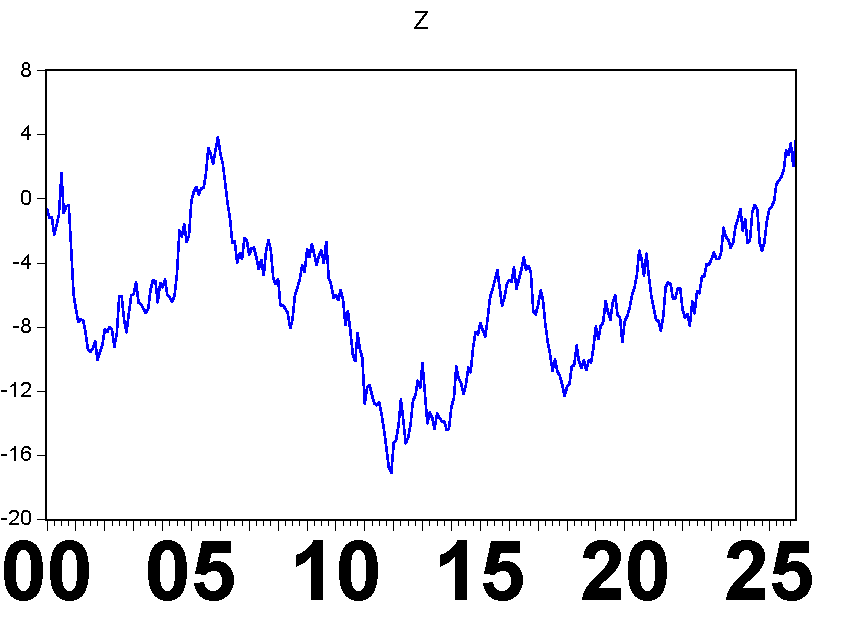
\includegraphics[width=0.45\textwidth]{test_engEviews_files/figure-latex//mychunk-grap1} }\subfloat[Another figure\label{fig:mychunk-2}]{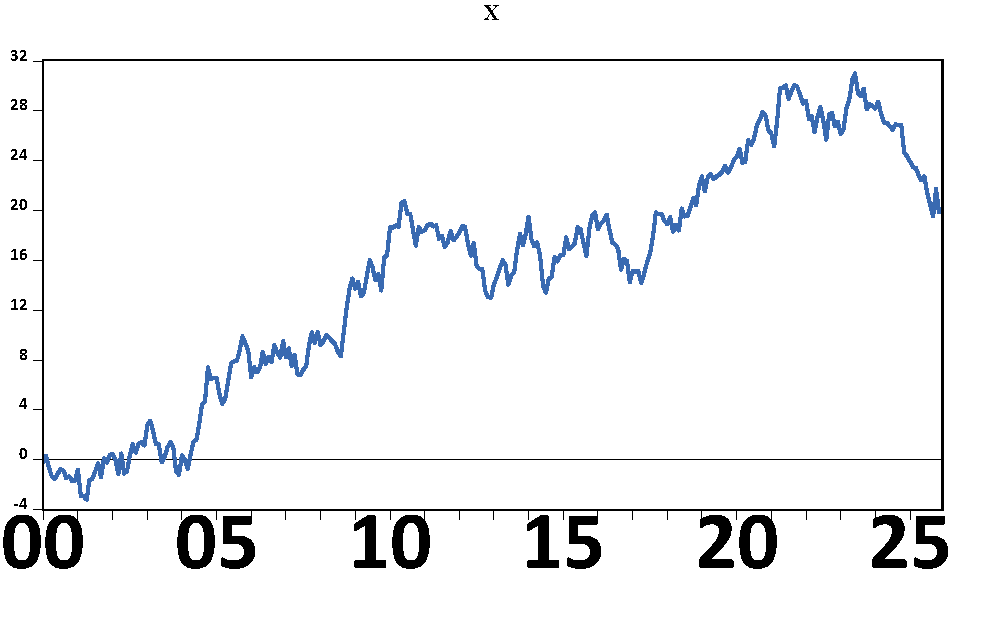
\includegraphics[width=0.45\textwidth]{test_engEviews_files/figure-latex//mychunk-grap2} }\newline\subfloat[A figure\label{fig:mychunk-3}]{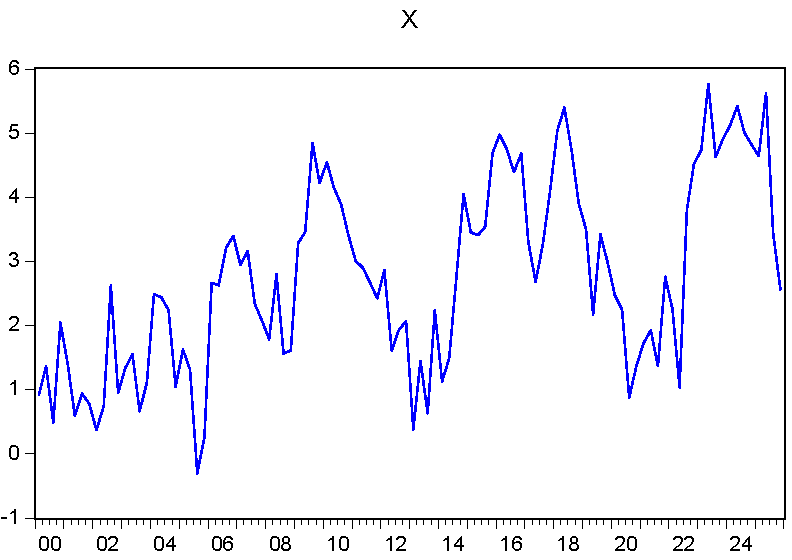
\includegraphics[width=0.45\textwidth]{test_engEviews_files/figure-latex//mychunk-grap} }

}

\caption{somefigure}\label{fig:mychunk}
\end{figure}

\begin{verbatim}
##        aic  df     coefs       dw        f    fprob       hq      logl  meandep
## 1 6.420486 102 -2.000060 0.040916 11.66674 0.000915 6.441088 -331.8653 3.185255
## 2       NA  NA -0.556338       NA       NA       NA       NA        NA       NA
##   ncoef     pval      r2    rbar2 regobs schwarz    sddep       se      ssr
## 1     2 0.221514 0.10264 0.093842    104 6.47134 6.240458 5.940437 3599.457
## 2    NA 0.000915      NA       NA     NA      NA       NA       NA       NA
##    stderrs    tstats
## 1 1.626021 -1.230033
## 2 0.162879 -3.415660
\end{verbatim}

\begin{verbatim}
## [1] 102
## attr(,"na.action")
## [1] 2
## attr(,"class")
## [1] "omit"
\end{verbatim}

\begin{verbatim}
##         date          x           y          z
## 1 2000-01-01  0.9573830  0.08212177  0.5195634
## 2 2000-04-01  0.5242838  1.57199365 -0.5714357
## 3 2000-07-01 -0.1000225  1.07387418 -0.8045620
## 4 2000-10-01 -2.3302412 -0.70266674  0.4728364
## 5 2001-01-01 -2.6229446 -0.21864240  1.0139448
## 6 2001-04-01 -1.7250749  0.24590107  1.8887011
\end{verbatim}

\hypertarget{r-plots}{%
\section{R plots}\label{r-plots}}

\begin{verbatim}
## NULL
\end{verbatim}

\begin{verbatim}
## [1] "asis"
\end{verbatim}

\begin{figure}[h]

{\centering 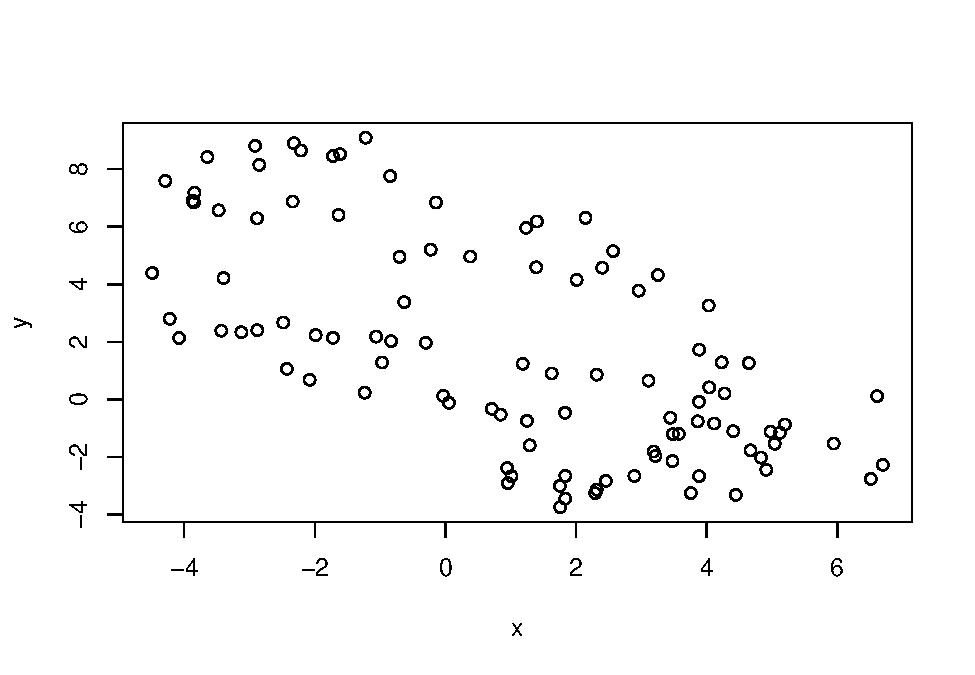
\includegraphics[width=0.45\textwidth]{test_engEviews_files/figure-latex/labe-1} 

}

\caption{another fig}\label{fig:labe}
\end{figure}

\begin{center}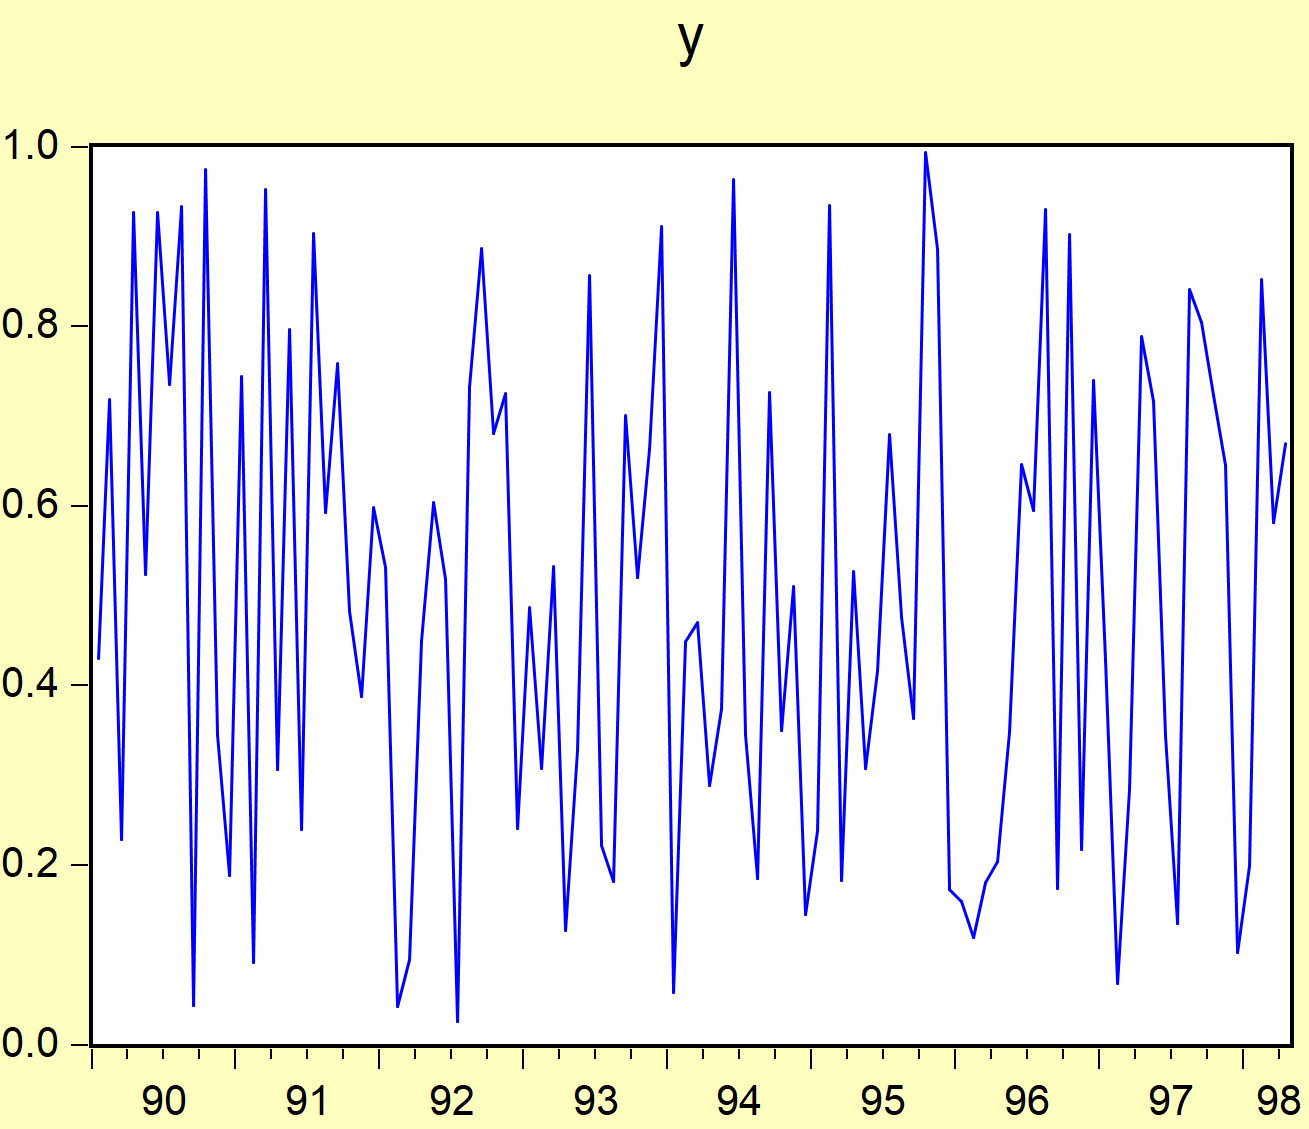
\includegraphics[width=0.45\textwidth]{test_engEviews_files/figure-latex//eview-graph-y} \end{center}

\begin{center}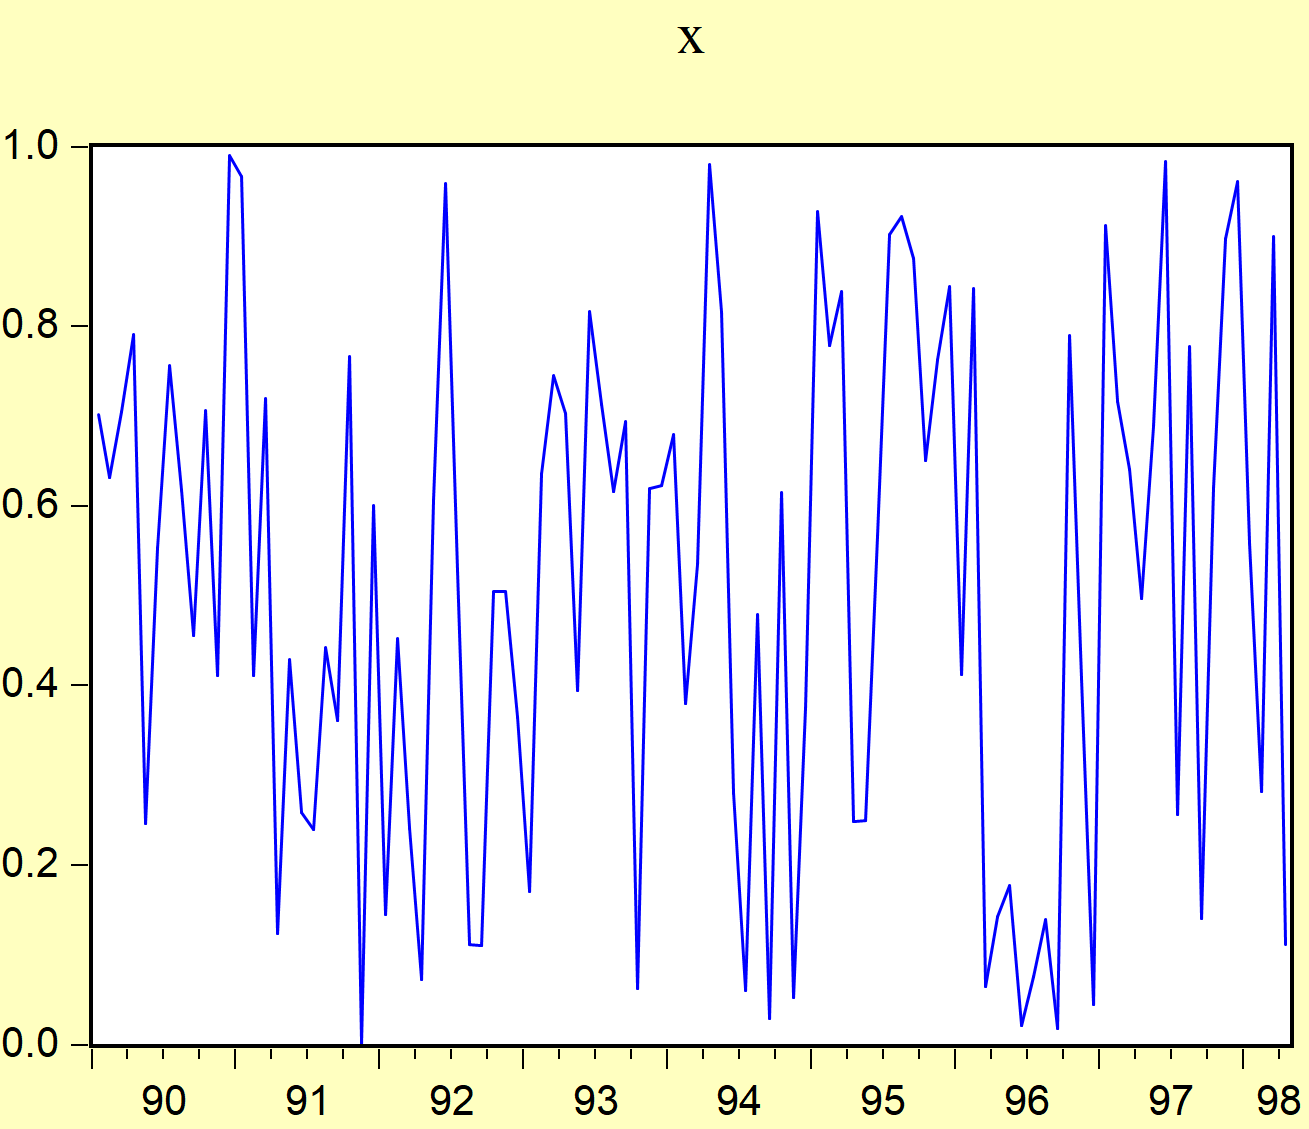
\includegraphics[width=0.45\textwidth]{test_engEviews_files/figure-latex//eview-graph-x} \end{center}

\begin{verbatim}
##         date        x          y        z
## 1 2001-01-01 2.480251 -0.1161992 1.696703
## 2 2001-01-02 1.747177 -0.2826314 2.926118
## 3 2001-01-03 1.166155 -0.6474547 3.852691
## 4 2001-01-04 1.961779 -0.5669765 4.357686
## 5 2001-01-05 3.142310 -1.3430673 5.298862
## 6 2001-01-06 3.042487 -1.1681385 3.631511
\end{verbatim}

\begin{center}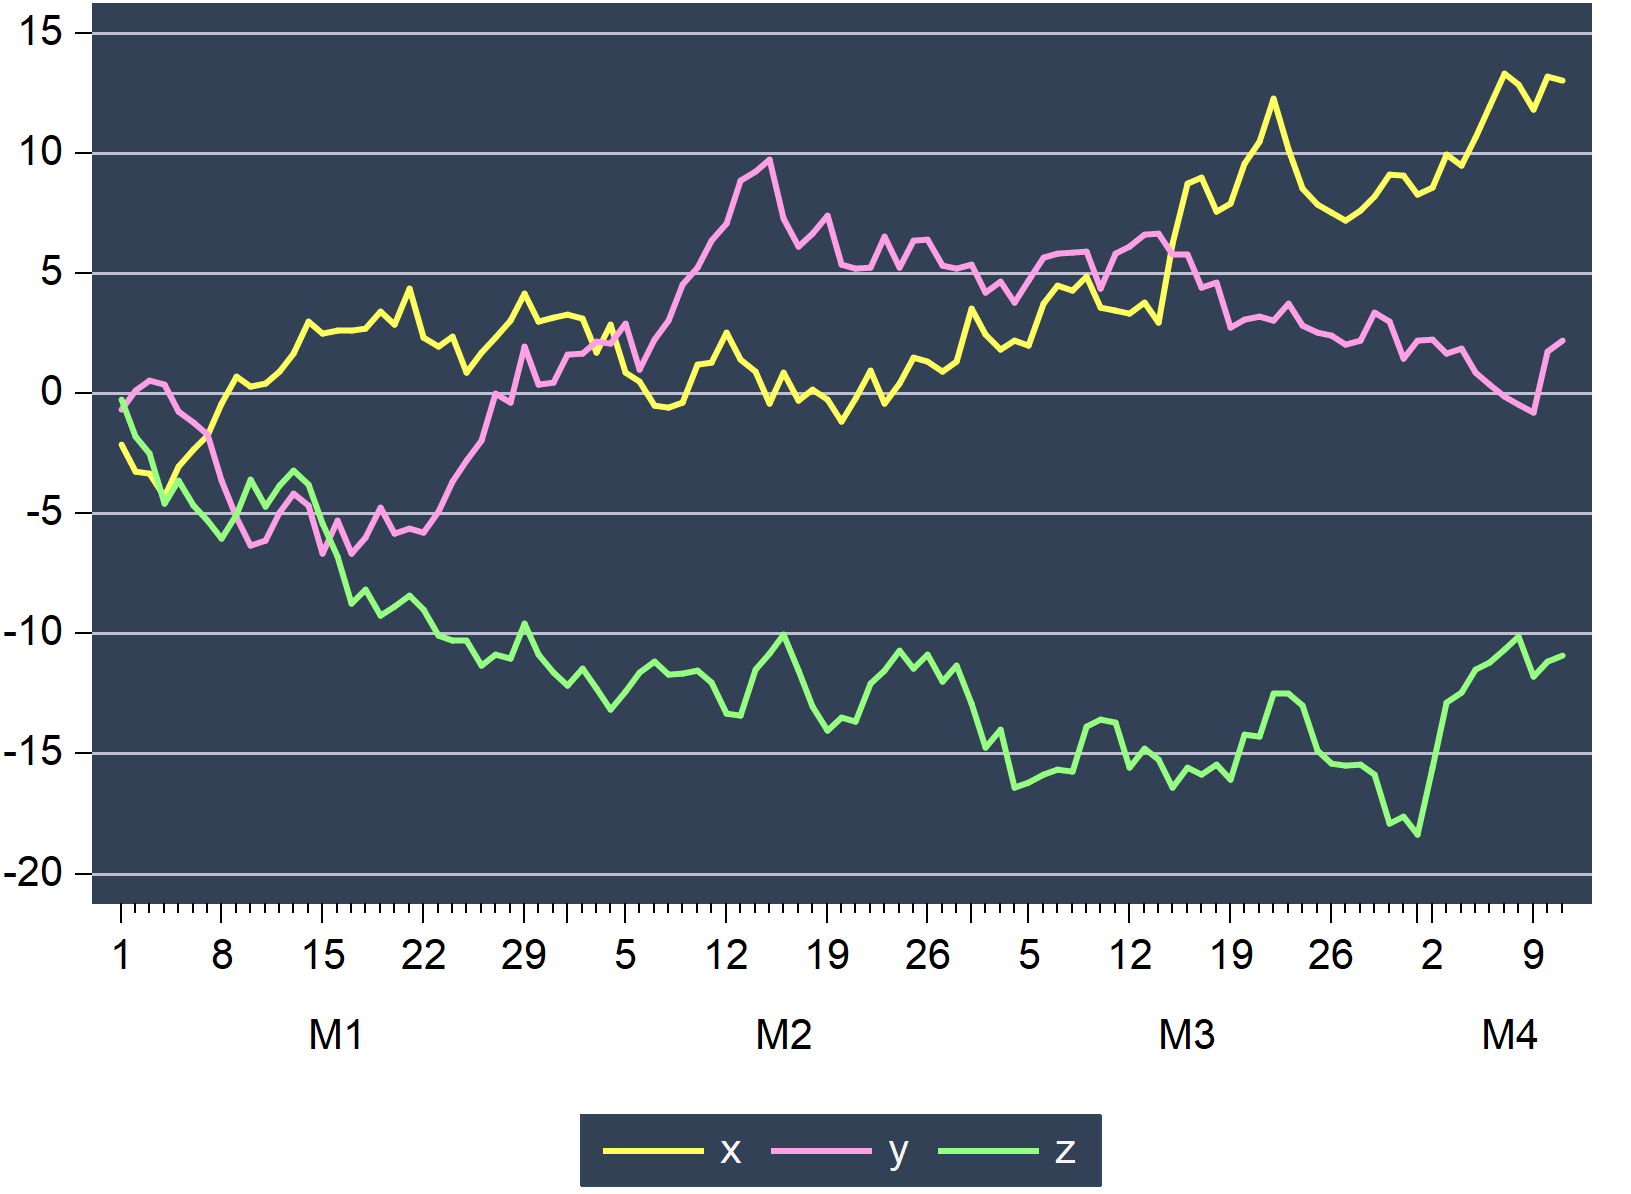
\includegraphics[width=0.45\textwidth]{test_engEviews_files/figure-latex//rwalk-xyz} \end{center}

\end{document}
